\documentclass[a4paper, 12pt]{article}
% packages
\usepackage{amssymb}
\usepackage[fleqn]{mathtools}
\usepackage{tikz}
\usepackage{enumerate}
\usepackage{bussproofs}
\usepackage{xcolor}
\usepackage[margin=1.3cm]{geometry}
\usepackage{logicproof}
\usepackage{diagbox}
\usepackage{karnaugh-map}
\usepackage{circuitikz}
\usetikzlibrary{arrows, shapes.gates.logic.US, calc, automata, positioning}

% augmented matrix
\makeatletter
\renewcommand*\env@matrix[1][*\c@MaxMatrixCols c]{%
\hskip -\arraycolsep
\let\@ifnextchar\new@ifnextchar
\array{#1}}
\makeatother

% ceiling / floor
\DeclarePairedDelimiter{\ceil}{\lceil}{\rceil}
\DeclarePairedDelimiter{\floor}{\lfloor}{\rfloor}

% custom commands
\newcommand{\indefint}[2]{\int #1 \, \mathrm{d}#2}
\newcommand{\defint}[4]{\int_#1^#2 #3 \, \mathrm{d}#4}
\newcommand{\dif}[2]{\frac{\mathrm{d}#1}{\mathrm{d}#2}}
\newcommand{\limit}[2]{\displaystyle{\lim_{#1 \to #2}}}
\newcommand{\summation}[3]{\sum\limits_{#1}^#2 #3}
\newcommand{\intbracket}[3]{\left[#3\right]_#1^#2}

\newcommand{\powerset}[0]{\wp}
\renewcommand{\emptyset}[0]{\varnothing}

\newcommand{\unaryproof}[2]{\AxiomC{#1} \UnaryInfC{#2} \DisplayProof}
\newcommand{\binaryproof}[3]{\AxiomC{#1} \AxiomC{#2} \BinaryInfC{#3} \DisplayProof}

% no indent
\setlength\parindent{0pt}

% reasoning proofs
\newcommand{\proofline}[3]{(#1)\ & #2 & \text{#3} \\}
\allowdisplaybreaks

% actual document
\begin{document}
    \section*{CO112 - Hardware}
        \subsection*{Prelude}
            The content discussed here is part of CO112 - Hardware (Computing MEng); taught by Bernhard Kainz, and Bjoern Schuller, in Imperial College London during the academic year 2018/19. The notes are written for my personal use, and have no guarantee of being correct (although I hope it is, for my own sake). This should be used in conjunction with the notes, and lecture slides. This course starts off fairly slow, especially if you have an idea of how logic gates work, and therefore the first parts won't be covered in much detail.
        \subsection*{Lecture 1}
            This section will be covered in less detail, as we've gone through the majority of this in much greater depth during logic. However, we will need to change the notation we use in this course from the one used in logic, from using $\land$ to $\cdot$, $\lor$ to $+$, and from $\neg$ to $^\prime$.
            \begin{center}
                \begin{tabular}{cc|c|c|c}
                    $A$ & $B$ & $A \cdot B$ (AND) & $A + B$ (OR) & $A^\prime$ (NOT) \\
                    \hline
                    0 & 0 & 0 & 0 & 1 \\
                    0 & 1 & 0 & 1 & 1 \\
                    1 & 0 & 0 & 1 & 0 \\
                    1 & 1 & 1 & 1 & 0
                \end{tabular}
            \end{center}
            The same distributivity laws apply, just like in \textbf{CO140}, as well as the simplification laws. In general, the laws should be the same as propositional logic, with the notation being slightly changed. Use 1 for $\top$, and 0 for $\bot$. We will also be using de Morgan's theorem on any number of variables (this can be proven by induction), such that $(V_1 + V_2 + V3 + ... + V_n)^\prime \equiv V_1^\prime \cdot V_2^\prime \cdot V_3^\prime \cdot ... \cdot V_n^\prime$, and the same the other way around. This can be very useful later on, as we will often use NAND / NOR gates to reduce silicon area.
        \subsection*{Lecture 2}
            The three operators covered in the first lecture can be represented by three logic gates; AND, OR, and NOT. The inverter (NOT), is represented by the circle at the end of the triangle. We can also create operations such as NAND, and NOR. Any of the first three gates can be built with just NAND gates, or just NOR gates. Let us represent $A$ NAND $B$, with $A \uparrow B$.
            \begin{itemize}
                \itemsep0em
                \item $A^\prime$ \hfill $A \uparrow A$
                \item $A \cdot B$ \hfill $(A \uparrow B)^\prime$
                    \subitem \hfill $(A \uparrow B) \uparrow (A \uparrow B)$
                \item $A + B$ \hfill $(A ^\prime \cdot B^\prime)^\prime$ (de Morgan's)
                    \subitem \hfill $A^\prime \uparrow B^\prime$
                    \subitem \hfill $(A \uparrow A) \uparrow (B \uparrow B)$
            \end{itemize}
            We also need to introduce two new gates, which are commonly used in digital logic; XOR, and XNOR. Roughly, you can use the same rules for $\neg (A \leftrightarrow B)$, and $A \leftrightarrow B$ respectively. XOR is commonly represented by $A \oplus B$ (which is much shorter than $A \cdot B^\prime + A^\prime \cdot B$), and XNOR represented by $(A \oplus B)^\prime$, instead of $A^\prime \cdot B^\prime + A \cdot B$. It has the following truth table;
            \begin{center}
                \begin{tabular}{cc|c|c}
                    $A$ & $B$ & $A \oplus B$ & $(A \oplus B)^\prime$ \\
                    \hline
                    0 & 0 & 0 & 1 \\
                    0 & 1 & 1 & 0 \\
                    1 & 0 & 1 & 0 \\
                    1 & 1 & 0 & 1
                \end{tabular}
            \end{center}
            In general, with $n$ inputs, we can have $2^n$ unique gates.
            With this information, we can build a single control block. For example, let there be a block with an input $A$, a control $C$, and output $R$. It follows that if $C$ is 0, then the output is 0, and $A$, if $C$ is 1. Hence $R = A \cdot C$.
            \medskip

            Now, if we had something with two inputs, $A$, and $B$, and a control $C$, we could use $C$ to determine whether $R = A$, or $R = B$. This is done with the boolean equation $R = A \cdot C^\prime + B \cdot C$. This is a \textbf{multiplexer}, which will be used very often in circuit design for other components.
        \subsection*{Lecture 3}
            Consider an more complex circuit, where we have 3 outputs; $R_1, R_2$, and $R_3$, and 4 inputs; $A, B, C$, and $D$, where $R_n=f_n(A, B, C, D)$. For now, we ignore sequential circuits, where the output can be on either side of the equation. The first step of creating a circuit is to construct a truth table as a starting point. We also need to define a few terms;
            \begin{itemize}
                \itemsep0em
                \item \textbf{minterm} - a boolean product where each input, or its complement, appears exactly once
                    \subitem hence $A \cdot B^\prime \cdot C$ is a minterm, but $A \cdot B$ isn't.
                    \subitem also known as sum-of-products, or disjunction-of-conjunctions
                \item \textbf{maxterm} - a boolean sum where each input, or its complement, appears exactly once
                    \subitem hence $A + B^\prime + C$ is a maxterm, but $A + B$ isn't.
                    \subitem also known as product-of-sums, or conjunction-of-disjunctions
            \end{itemize}
            For example, let's work on the following truth table;
            \begin{center}
                \begin{tabular}{c|c|c|c|c}
                    $A$ & $B$ & $C$ & $R$ & \\
                    \hline
                    0 & 0 & 0 & 0 & maxterm $A + B + C$ \\
                    0 & 0 & 1 & 0 & maxterm $A + B + C^\prime$ \\
                    0 & 1 & 0 & 0 & maxterm $A + B^\prime + C$ \\
                    0 & 1 & 1 & 1 & minterm $A \cdot B \cdot C$ \\
                    1 & 0 & 0 & 0 & maxterm $A^\prime + B + C$ \\
                    1 & 0 & 1 & 1 & minterm $A \cdot B^\prime \cdot C$ \\
                    1 & 1 & 0 & 1 & minterm $A \cdot B \cdot C^\prime$ \\
                    1 & 1 & 1 & 1 & minterm $A \cdot B \cdot C$
                \end{tabular}
            \end{center}
            Now, we can evaluate $R$ in two ways;
            \begin{itemize}
                \itemsep0em
                \item $R = (A \cdot B \cdot C) + (A \cdot B^\prime \cdot C) + (A \cdot B \cdot C^\prime) + (A \cdot B \cdot C)$ \hfill sum of minterms
                \item $R = (A + B + C) \cdot (A + B + C^\prime) \cdot (A + B^\prime + C) \cdot (A^\prime + B + C)$ \hfill product of maxterms
            \end{itemize}
            Knowing this, we can convert any truth table into a \textbf{Karnaugh map}
            \begin{center}
                \begin{tabular}{c|c|c|c|c||c|c|c|c|c}
                    $A$ & $B$ & $C$ & $D$ & $R$ & $A$ & $B$ & $C$ & $D$ & $R$ \\
                    \hline
                    0 & 0 & 0 & 0 & 0 & 1 & 0 & 0 & 0 & 1 \\
                    0 & 0 & 0 & 1 & 1 & 1 & 0 & 0 & 1 & 1 \\
                    0 & 0 & 1 & 0 & 1 & 1 & 0 & 1 & 0 & 1 \\
                    0 & 0 & 1 & 1 & 1 & 1 & 0 & 1 & 1 & 1 \\
                    0 & 1 & 0 & 0 & 0 & 1 & 1 & 0 & 0 & 1 \\
                    0 & 1 & 0 & 1 & 1 & 1 & 1 & 0 & 1 & 1 \\
                    0 & 1 & 1 & 0 & 1 & 1 & 1 & 1 & 0 & 1 \\
                    0 & 1 & 1 & 1 & 0 & 1 & 1 & 1 & 1 & 1
                \end{tabular}

                \begin{karnaugh-map}[4][4][1][$CD$][$R:\ AB$]
                    \manualterms{0, 1, 1, 1, 0, 1, 1, 0, 1, 1, 1, 1, 1, 1, 1, 1}
                    \implicant{12}{10}
                    \implicant{1}{9}
                    \implicant{3}{2}
                    \implicant{6}{6}
                \end{karnaugh-map}
            \end{center}
            Hence we can use minterms, to get $R = \underbrace{A}_\text{red} + \underbrace{C^\prime \cdot D}_\text{green} + \underbrace{A^\prime \cdot B^\prime \cdot C}_\text{yellow} + \underbrace{A^\prime \cdot B \cdot C \cdot D^\prime}_\text{blue}$. 
            \medskip

            Remember that the regions in the map can wrap around, and that don't cares can count as either 0, or 1.
        \subsection*{Lecture 4}
            A general circuit can be used to generate all possible $n$-input digital circuits. If we were to have inputs $V_1, V_2, ..., V_n$, and have each one come out as two lines, so $V_i$ would come out with $V_i$, and its complement $V_i^\prime$. We can have $2^n$ $n$-input AND gates, which correspond to each possible combination (00...00), (00...01), (00...11), all the way to (11...11). This is hard to visualise (see \textit{Notes04 - Description to Circuit.pdf}), but the general idea is that each AND gate corresponds to a possible minterm, which is joined to a $2^n$-input OR gate, if it's a 1 in the truth table. This is a \textbf{Programmable Array Logic (PAL)} device, and the device can be programmed by sending a current through specific links to connect them to the OR gate.
            \medskip

            The general steps for creating a device from a specified device are as follows;
            \begin{enumerate}[1.]
                \itemsep0em
                \item Construct a truth table
                    \subitem translate the natural language description of what the device should do into a truth table.
                \item Generate a Karnaugh map
                    \subitem using the techniques mentioned in the previous lecture, create the map, and find the resulting sum of minterms (or product of maxterms)
                \item Minimise the boolean expression
                    \subitem using the resulting sum or product, we can then use boolean algebra to simplify the expression
                \item Design the circuit
                    \subitem using the minimised boolean expression, we can finally construct a circuit
                \item Minimise the circuit
                    \subitem this is different from minimising the equation, as we're now trying to minimise the silicon area used
                    \subitem in general, this is to replace ANDs, and ORs, with NANDs, and NORs
                    \subitem a method of doing this is to replace expressions such as $(A \cdot B)$ with $(A^\prime + B^\prime)^\prime$, by using de Morgan's law
                \item Test the circuit
                    \subitem the usual process is to simulate the circuit, to validate it against the original specifications
                    \subitem finding bugs before production is important (and expensive, if not spotted); see the \textit{Floating Point Division Bug} in \textit{Intel Pentium P5}
            \end{enumerate}
        \subsection*{Lecture 5}
            While boolean algebra is a good abstraction for the behaviour of logic gates, it has some subtle differences, which can be problematic, and cause bugs. Practically, voltages aren't exact values, and therefore thresholds have to be arbitrarily determined - leading to more issues (such as what happens when the voltage is between the lower, and upper threshold). The main difference is that boolean algebra doesn't consider time delays, which exist despite electrons moving at light-speed. This failure to synchronise events is a common error in hardware design, and therefore we will require a more accurate physical model (note that all models are simply approximations, but we should choose one of a sensible degree of accuracy).
            \medskip

            To define the physical representation of a logic gate, we'll need to reuse some components from A Level Physics.
            \begin{itemize}
                \itemsep0em
                \item components
                    \subitem resistor
                    \subitem capacitor
                    \subitem transistor
                \item equations
                    \subitem $V = I \cdot R$ \hfill Ohm's law
                    \subitem $I = C\dif{V}{t}$ \hfill Capacitance
            \end{itemize}
            Pure silicon is an extremely good insulator, however if we were to infuse (\textbf{dope}) it with impurities to give it surplus electrons, it would then be able to conduct electricity; this type of semiconductor is known as \textbf{n-type}. On the other hand, if we were to infuse it with positive charge carriers (which would just be holes, with missing electrons), we'd have \textbf{p-type}. A transistor is made of three adjacent pieces of these semiconductors; and can either be \textbf{n-p-n}, or \textbf{p-n-p}. While Ohm's law is a simple mathematical method for resistors, and it's possible to derive a set of equations for more complex devices, we're engineers. We will consider the transistor as a switch (as a set of rules, called a procedural model).
            \medskip

            Consider the transistor as a switch with three terminals; a source $S$, a drain $D$, and a gate $G$. There is no connection between $G$, and $S$, nor is there a connection between $G$, and $D$. If the voltage between $G$, and $S$ (let it be $V_{GS}$) $\leq 0.5\mathrm{v}$, there is no connection between $S$, and $D$. On the other hand, if $V_{GS} \geq 1.7\mathrm{v}$, then $S$ is connected to $D$, and therefore current can flow through. In an ideal world, when the switch is closed, it has 0 resistance, and when it is open, the resistance is $\infty$ (this isn't correct, for reasons that will be discussed later).
            \medskip

            In general, if there is a high resistance (the circuit is broken), then the output is high (since we have (almost) no current flowing, $I \approx 0$, therefore the P.D. across the resistor, $V_\text{R} \approx 0$), and $V_\text{out} \approx 5$. However, if it is connected, we will consider it to have a very low resistance, hence the larger P.D. would be across the resistor, thus having a lower $V_\text{out}$.
            \medskip

            The physical representation of logic gates explains why NAND, and NOR gates are cheaper, as they each only require two transistors (in series, or in parallel, respectively).
            \medskip

            There are two main reasons for why there are time delays in a circuit. The first is the state change of the transistor; the electrons will still take time to move through it. Second is the representation of the transistor; we need to consider the transistor as more of a variable resistor. By reducing the size of the capacitor, we have a lower capacitance, and hence a faster charge. We can calculate a formula for voltage over time; (note that $K = -\mathrm{ln}(5)$, since $V(0) = 0$)
            \begin{align*}
                5 - V & = I \cdot R \\
                I & = C \dif{V}{t} \\
                5 - V & = RC \dif{V}{t} \\
                \frac{5 - V}{\mathrm{d}V} & = \frac{RC}{\mathrm{d}t} \\
                \indefint{\frac{1}{5 - V}}{V} & = \indefint{\frac{1}{RC}}{t} \\
                -\mathrm{ln}(5 - V) & = \frac{t}{RC} + K \\
                -\mathrm{ln}(5 - V) & = \frac{t}{RC} - \mathrm{ln}(5) \\
                \mathrm{ln}(5 - V) & = \mathrm{ln}(5) - \frac{t}{RC} \\
                5 - V & = e^{\mathrm{ln}(5) - \frac{t}{RC}} \\
                5 - V & = e^{\mathrm{ln}(5)} \cdot e^{-\frac{t}{RC}} \\
                5 - V & = 5e^{-\frac{t}{RC}} \\
                V & = 5 - 5e^{-\frac{t}{RC}} \\
                V & = 5(1 - e^{-\frac{t}{RC}})
            \end{align*}
        \subsection*{Lecture 6}
            Consider the case where we have a NAND gate, with inputs $A$, and $R$ (which is coming from the output $R$). When $A = 1$, we have $R = (A \cdot R)^\prime = (1 \cdot R)^\prime = R^\prime$; which is clearly inconsistent. This is where the logic breaks down - however in real life, there's nothing stopping us from doing this. Continuing on from the previous lecture, we have two models;
            \begin{itemize}
                \itemsep0em
                \item \textbf{Switch and Delay}
                    \subitem only differs from boolean algebra due to the inclusion of a time delay between the change in the input, and the change in the output
                \item \textbf{Resistance and Capacitance}
                    \subitem this is a more accurate representation of real behaviour, and during the time delay period, it's no longer a valid boolean signal
                    \subitem this is a analogue model, and not digital (digital electronics don't actually exist, due to noise, and therefore we use safety margins) - for example, a voltage above 1.7v would be logic 1, and a voltage between 0.5v would be logic 0
            \end{itemize}
            Despite defining the noise margins above, we should design our circuits so that they operate far from the thresholds, such that we can have boolean 1 around 3.5v, and boolean 0 at around 0.3v. Since we're considering the transistor as a variable resistor, it acts like a potential divider.
            \medskip

            Remembering from physics, we can take $\frac{1}{R_\text{total}} = \frac{1}{R_\text{var}} + \frac{1}{R_\text{load}}$, and therefore calculate $V_\text{out} = \frac{5R_\text{total}}{R_\text{source} + R_\text{total}}$. Here, $R_\text{load}$ is the combined resistance of all gates the transistor is connected to.
            \begin{center}
                \begin{circuitikz}
                    \node[] (5v) at (0, 4) {5v};
                    \node[] (vout) at (3, 2) {$V_\text{out}$};
                    \draw
                    (5v) -- (1.5, 4)
                    (0.75, 2) -- (vout)
                    (0, 0) -- (3, 0)
                    (0.75, 4) to[R, l=$R_\text{source}$] (0.75, 2)
                    (0.75, 0) to[R, l=$R_\text{var}$] (0.75, 2)
                    (1.5, 2) to[R, l=$R_\text{load}$] (1.5, 0);
                \end{circuitikz}
                $\equiv$
                \begin{circuitikz}
                    \node[] (5v) at (0, 4) {5v};
                    \node[] (vout) at (3, 2) {$V_\text{out}$};
                    \draw
                    (5v) -- (1.5, 4)
                    (0.75, 2) -- (vout)
                    (0, 0) -- (3, 0)
                    (0.75, 4) to[R, l=$R_\text{source}$] (0.75, 2)
                    (0.75, 2) to[R, l=$R_\text{total}$] (0.75, 0);
                \end{circuitikz}
            \end{center}
            As we know the inverse law for parallel resistors, we can say the load resistance $R_\text{load}$ becomes $\frac{1}{n}$ of a single gate, when there are $n$ identical gates connected to a single gate output. Not only does this \textbf{fan-out} cause issues with the thresholds, we also need to consider the time delay. The time delay is directly proportional to the size of the load capacitor (trivial to derive from the equations listed), and capacitors in parallel add up, hence a larger fan-out would have a larger time delay. For the time being, we will stick to the original \textbf{switch-and-delay} model.
            \medskip

            Going back to the problem at hand, with the NAND gate, we would have an extremely high frequency oscillation. If we construct a table for the states, we can determine which states are stable. This effect can be harnessed to make memory.
        \subsection*{Lecture 7}
            I will use the following notation for stating the values of inputs; $I_1...I_n(v_1, ..., v_n)$ means that $I_i = v_i\ \forall i \in [1, n]$; so $SR(1, 0)$ would mean $S = 1$, and $R = 0$.
            \medskip

            Looking at the states for the \textbf{R-S flip flop}, we can get the following states;
            \begin{center}
                \begin{tabular}{c|c||c|c|c|c}
                    $S$ & $R$ & $P_t$ & $Q_t$ & $P_{t+1}$ & $Q_{t+1}$ \\
                    \hline
                    0 & 0 & $\times$ & $\times$ & 1 & 1 \\
                    0 & 1 & $\times$ & $\times$ & 1 & 0 \\
                    1 & 0 & $\times$ & $\times$ & 0 & 1 \\
                    1 & 1 & 0 & 0 & 1 & 1 \\
                    1 & 1 & 0 & 1 & 0 & 1 \\
                    1 & 1 & 1 & 0 & 1 & 0 \\
                    1 & 1 & 1 & 1 & 0 & 0
                \end{tabular}
            \end{center}
            You might be able to notice that when $SR(1, 1)$, and $P = Q^\prime$, we have a stable state. In general, we have $P = Q^\prime$, as long as we reset the flip-flop, and avoid $RS(0, 0)$. Looking at the $RS(1, 1)$ state, where it's bi-stable, it can theoretically oscillate infinitely, but in practice the gates will likely have different time delays, and will therefore fall into a stable state. As we have this uncertainty, we send a reset signal $RS(0, 1)$, which sets the $Q$ to 1, and after that point we have predictable behaviour (given we avoid $RS(0, 0)$). This way, we will be able to get $RS(0, 1) \to Q = 1$, and $RS(1, 0) \to Q = 0$. However, this mechanism isn't convenient for practical memory circuits, so we adapt it with a latch. This way, if the latch is engaged ($L = 1$), we set $Q = D$.
            \begin{center}
                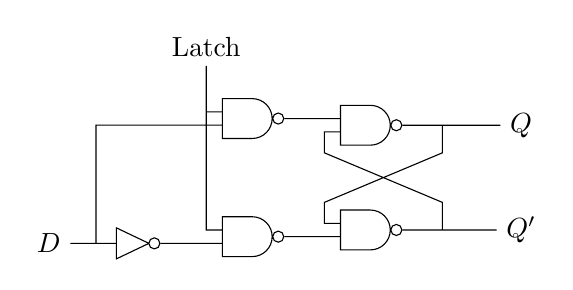
\begin{tikzpicture}[y=-1cm]
                    \node (L) at (2, -2.5) {Latch};
                    \node (D) at (0, 0) {$D$};

                    \node[not gate US, draw] (notD) at ($(D) + (1, 0)$) {};
                    \node[nand gate US, draw, logic gate inputs=nn] (nand1) at ($(notD) + (1.5, -0.085)$) {};
                    \node[nand gate US, draw, logic gate inputs=nn] (nand2) at ($(nand1) + (0, -1.5)$) {};
                    \node[nand gate US, draw, logic gate inputs=nn] (nand3) at ($(nand1) + (1.5, -0.085)$) {};
                    \node[nand gate US, draw, logic gate inputs=nn] (nand4) at ($(nand2) + (1.5, 0.085)$) {};

                    \node (Qp) at ($(nand3) + (2, 0)$) {$Q^\prime$};
                    \node (Q) at ($(nand4) + (2, 0)$) {$Q$};

                    \draw
                    (D) -- (notD.input)
                    ($(D) + (0.6, 0)$) |- (nand2.input 2)
                    (notD.output) -- (nand1.input 2)
                    (L) |- (nand1.input 1)
                    (L) |- (nand2.input 1)
                    (nand1.output) -- (nand3.input 2)
                    (nand2.output) -- (nand4.input 1)
                    (nand3.output) -- (Qp)
                    (nand4.output) -- (Q)
                    (nand3.input 1) -| ($(Qp) + (-2.5, -0.35)$) -- ($(Q) + (-1, 0.35)$) -- ($(Q) + (-1, 0)$)
                    (nand4.input 2) -| ($(Q) + (-2.5, 0.35)$) -- ($(Qp) + (-1, -0.35)$) -- ($(Qp) + (-1, 0)$);
                \end{tikzpicture}
            \end{center}
            However; there would be a time delay, as the NOT gate would introduce a small delay. We can get around this by using a \textbf{Master-Slave Flip-Flop}, which combines two D Flip-Flops, thus allowing for $Q$ to only be set on the \textbf{falling edge} of the clock signal.
            \begin{center}
                \begin{tikzpicture}
                    \node (clock) at (0, 0) {Clock};
                    \node (d) at (0, -1.5) {$D$};
                    \node (q) at (7.5, -1.5) {$Q$};
                    \node (qp) at (7.5, -3.2) {$Q^\prime$};
                    \node[not gate US, draw] (notclock) at (3.7 , 0) {};

                    \draw
                    (1, -1.1) -- (2.5, -1.1) -- (2.5, -3.6) -- (1, -3.6) -- cycle
                    (5, -1.1) -- (6.5, -1.1) -- (6.5, -3.6) -- (5, -3.6) -- cycle
                    (2.5, -1.5) -- (5, -1.5)
                    (2.5, -3.2) -- (3, -3.2)
                    (d) -- (1, -1.5)
                    (q) -- (6.5, -1.5)
                    (qp) -- (6.5, -3.2)
                    (clock) -- (notclock.input)
                    (notclock.output) -- (5.75, 0) -- (5.75, -1.1)
                    (1.75, 0) -- (1.75, -1.1);
                \end{tikzpicture}
            \end{center}
            While we don't have to memorise the circuit diagrams of all the flip-flops for the exam, it's important to remember the state diagrams;
            \begin{itemize}
                \itemsep0em
                \item D-Type Flip-Flop
                    \begin{center}
                        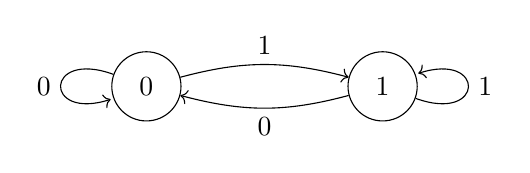
\begin{tikzpicture}
                            \node[state] (0) at (0, 0) {0};
                            \node[state] (1) at (3, 0) {1};

                            \draw
                            (0) edge[bend left=15, above, ->] node{1} (1)
                            (1) edge[bend left=15, below, ->] node{0} (0)
                            (0) edge[out=160, in=200, loop, left] node{0} (0)
                            (1) edge[out=-20, in=20, loop, right] node{1} (1);
                        \end{tikzpicture}
                    \end{center}
                \item T-Type Flip-Flop
                    \begin{center}
                        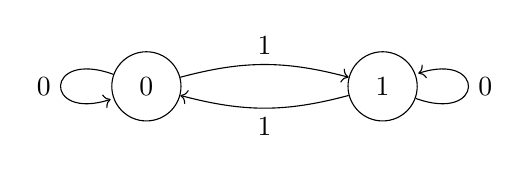
\begin{tikzpicture}
                            \node[state] (0) at (0, 0) {0};
                            \node[state] (1) at (3, 0) {1};

                            \draw
                            (0) edge[bend left=15, above, ->] node{1} (1)
                            (1) edge[bend left=15, below, ->] node{1} (0)
                            (0) edge[out=160, in=200, loop, left] node{0} (0)
                            (1) edge[out=-20, in=20, loop, right] node{0} (1);
                        \end{tikzpicture}
                    \end{center}
                \item J-K Flip-Flop
                    \begin{center}
                        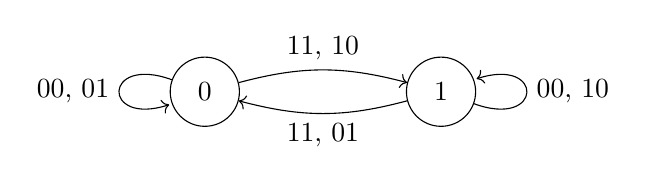
\begin{tikzpicture}
                            \node[state] (0) at (0, 0) {0};
                            \node[state] (1) at (3, 0) {1};

                            \draw
                            (0) edge[bend left=15, above, ->] node{11, 10} (1)
                            (1) edge[bend left=15, below, ->] node{11, 01} (0)
                            (0) edge[out=160, in=200, loop, left] node{00, 01} (0)
                            (1) edge[out=-20, in=20, loop, right] node{00, 10} (1);
                        \end{tikzpicture}
                    \end{center}
                    \subitem this is very useful, as it is able to store memory when you have $JK(0, 0)$, since it doesn't change state on that input
            \end{itemize}
        \subsection*{Lecture 8}
            The content covered in this lecture, is done in Coursework 2, and as such, I will be skipping over a lot of things. In general, if we have $k$ states, we will need to use $n = \ceil{\mathrm{log}_2(k)}$ D-type flip-flops, all connected to the same clock. A general synchronous sequential system would consist of a block of state sequencing logic, which takes in a set of $m$ inputs, as well as the current states of the flip-flops, and has $n$ outputs. The system would also need a block of output logic, which decodes the states into the appropriate outputs. In general, we can say that $Q_i = D_i(I_1, ..., I_m, Q_{1_\text{old}}, ..., Q_{n_\text{old}})\ \forall i \in [1..n]$, where $Q_i$ the updated state of the $i^\text{th}$ flip-flop.
            \medskip

            The J-K flip-flop is a very simple example of such a synchronise circuit, which is detailed above.
            \medskip

            In general, if we have "don't cares", we will consider them a logic 1 if they are inside any regions inside a Karnaugh map, and 0 otherwise. While components inside the Karnaugh map don't know about each other, we can reuse components when we implement our circuit in order to save silicon space.
        \subsection*{Lecture 9}
            The general notation we will be using is $S(t)$, or $S_t$ to represent $S$ at time $t$. We cover two main types of finite state machines in this course;
            \begin{itemize}
                \itemsep0em
                \item notation
                    \subitem $S$ = state of D-Q flip-flops
                    \subitem $O$ = output(s)
                    \subitem $I$ = input(s)
                    \subitem $f$ = input / sequencing logic
                    \subitem $g$ = output / decode logic
                \item Mealy Machine
                    \subitem $S(t + 1) = f(S(t), I(t))$
                    \subitem $O(t + 1) = g(S(t), I(t))$
                \item Moore Machine
                    \subitem $S(t + 1) = f(S(t), I(t))$
                    \subitem $O(t) = g(S(t))$
            \end{itemize}
            A synchronous digital circuit avoids time issues by having a bank of D-Q flip-flops (with a common clock), acting as a barrier between the input, and output. However, spikes can still occur in a Mealy machine, as the output is also controlled by the input. In general, the method for designing a synchronous circuit is as follows;
            \begin{enumerate}[1.]
                \itemsep0em
                \item determine the number of states
                \item determine the state transitions (and draw FSM)
                \item choose how the states are represented by the flip-flops
                \item express the state sequencing logic, and minimise said logic with Karnaugh maps
                \item express the output logic as a function of the states, minimising if possible
            \end{enumerate}
            There's an example in the notes, and in the lecture, but once again this is covered mostly in Coursework 2, and therefore will be skipped here.
        \subsection*{Lecture 10}
            Once again, the content from this lecture is covered in the coursework. However, it's important to note how to notice problems with the "don't care" states. In the slides, you'll see an example where the FSM gets stuck in a state, when we replace the "don't cares" with 1s or 0s, depending on whether they're in any Karnaugh map region, or not, respectively. To fix this, we find the offending line, and make a small change that will fix the bug, without adding too much additional bulk to the circuit. This is fixing by hacking.
        \subsection*{Lecture 11}
            Registers are fast, small bits of memory that are very accessible. An example of a register is the bank of D-Q flip-flops in the synchronous circuit., which can store an integer in the range $[-2^{n - 1}, 2^{n - 1} - 1]$, or $[0, 2^n - 1]$, depending on whether a sign is being used. However, we frequently use serial data, and not just parallel, in real life. For example, cables are often serial as it reduces size, and minimises the chance of cable failure. However in practice, data is often processed in parallel in a computer to increase speed, therefore conversion between the two types of data is required. The same circuit can be used for doing parallel-to-serial, and serial-to-parallel, being toggled by a multiplexer
            \medskip

            This method for loading serial data can be slow (due to the capacitance of the wires), especially with a larger set of data. Serial communication cannot be done as quickly as operations within the processor, which is why it is normally run on a separate clock, and utilises control lines to indicate when conversions are complete.
            \medskip

            This register can also be used for division, and multiplication, by 2. By increasing the number of functions our shift register has, we need to implement a more complex multiplexer. First we have to create a binary to unary converter, which converts an $n$-bit input, to a $2^n$ separate lines. This can then easily be combined with $n$ AND gates, and a single OR to select between $2^n$ inputs.
            \medskip

            We can use this to half the frequency of a clock, by connecting $Q^\prime$ into $D$. This will create the following square wave;
            \begin{center}
                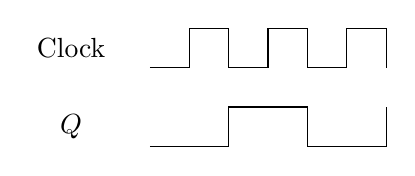
\begin{tikzpicture}
                    \node[] at (0, 0) {Clock};
                    \node[] at (0, -1) {$Q$};
                    \draw
                    (1, -0.25) -- (1.5, -0.25) -- (1.5, 0.25) -- (2, 0.25) -- (2, -0.25) -- (2.5, -0.25) -- (2.5, 0.25) -- (3, 0.25) -- (3, -0.25) -- (3.5, -0.25) -- (3.5, 0.25) -- (4, 0.25) -- (4, -0.25)
                    (1, -1.25) -- (2, -1.25) -- (2, -0.75) -- (3, -0.75) -- (3, -1.25) -- (4, -1.25) -- (4, -0.75);
                \end{tikzpicture}
            \end{center}
            This can then be easily chained to do divisions by powers of 2. However, only being able to divide by pwoers of 2 isn't exactly useful, and therefore division by other numbders is also important. By using a ripple through counter, we can count to a number, and then send a pulse on that tick, and then clear the memory, thus allowing us to divide by any integer. This counter however, is \textbf{not} synchronous. For example, if we wanted to divide by 5, we'd have $O = b_0 \cdot b_1^\prime \cdot b_2$, which would also feed into the top, as a clear signal.
            \begin{center}
                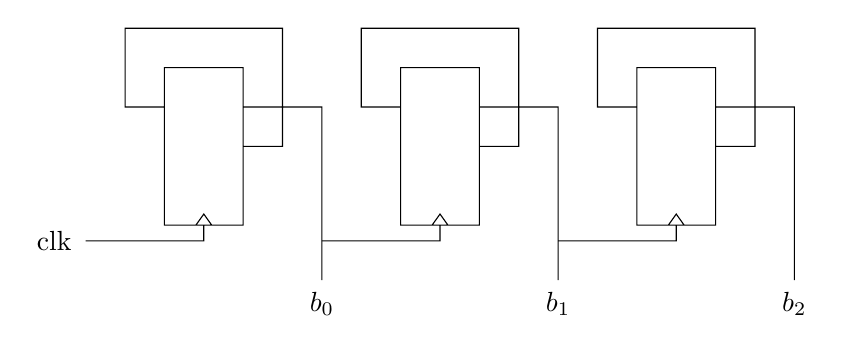
\begin{tikzpicture}
                    \node[] at (-1.4, -2.2) {clk};
                    \node[] at (2, -3) {$b_0$};
                    \node[] at (5, -3) {$b_1$};
                    \node[] at (8, -3) {$b_2$};

                    \foreach \x in {0,...,2} {
                        \draw
                        (3*\x, 0) -- (1 + 3*\x, 0) -- (1 + 3*\x, -2) -- (3*\x, -2) -- cycle

                        (0.4 + 3*\x, -2) -- (0.5 + 3*\x, -1.86) -- (0.6 + 3*\x, -2)

                        (-1 + 3*\x, -2.2) -| (0.5 + 3*\x, -2)
                        (1 + 3*\x, -0.5) -| (2 + 3*\x, -2.7)
                        (1 + 3*\x, -1) -| (1.5 + 3*\x, 0.5) -| (-0.5 + 3*\x, -0.5) -- (3*\x, -0.5);
                    }
                \end{tikzpicture}
            \end{center}
        \subsection*{Lecture 12}
            There's a lot of diagrams in this, so just look at \textit{Notes12 - Multiplexers.pdf} - TikZ is too painful.
            \medskip

            While we can build more optimised circuits, calculating the optimal solution is often not feasible, especially as the number of inputs grow (since the possible situations grow exponentially). In order to do this, we will reuse components - this is known as funcitonal design. Often, this will be done with the use of an Enable input, which in reality is just an additional AND gate right at the end.
            \medskip

            Something that will be needed often in a computer is transferring data between two registers. This is done in the following steps;
            \begin{enumerate}[1.]
                \itemsep0em
                \item select the input register (source)
                    \subitem on a machine with $n$ registers, this will be done on a $n$-1 multiplexer; the inputs of the multiplexer are the $Q$s of the registers (note that in the diagrams, a line with a slash running across it, and a number above, means that it has a certain number of wires - it's a bus)
                    \subitem the output of the multiplexer goes into $D$ for every register
                \item select the output register (destination)
                    \subitem you'll notice in the step above, it connects to every register - remember that a register only sets $Q$ to $D$, on the falling / rising edge of a clock
                    \subitem the clock is connected to the enable line of a demultiplexer (which is also known as a decoder), and the outputs of the demultiplexer are connected to the clock input for each corresponding register
                \item the data is then transferred on the clock edge
                    \subitem this is commonly written as $R_\text{destination} \leftarrow R_\text{source}$
            \end{enumerate}
            One of the most important circuits is the comparator; which compares values in two registers ($A$, and $B$), and gives an output depending on; $A > B$, $A = B$, or $A < B$. In reality, only two of those are needed, as the missing one is the NOR of the other two, whichever one we decide to drop is arbitrary. See the diagrams in the notes, since I've had enough of drawing them in TikZ for today.
        \subsection*{Lecture 13}
            \subsubsection*{Addition}
                First consider the half-adder; we have 3 inputs; $A$, $B$, and $C_\text{in}$, which is the carry bit. We also have 2 outputs; $S$, the sum, and $C_\text{out}$, which is the bit carried to the next most significant bit. This is trivial to represent as a truth table, so that will be skipped. We can say $C_\text{out} = A \cdot B$, and $S = A \oplus B$. We can also make a full-adder with two half-adders, this is done by having the $A_2 = S_1$, and $B_2 = C_{1_\text{out}}$. From this, we can get $S_2$ (the final sum), to be $S = S_1 \oplus C_\text{in} = A \oplus B \oplus C_\text{in}$, and $C_\text{out}$ (the final carry bit), to be $C_\text{out} = C_{1_\text{out}} + (S_1 \cdot C_\text{in}) = (A \cdot B) + C_\text{in} \cdot (A \oplus B)$.
                \medskip

                An $n$-bit full adder chains together $n$ full-adders, with a carry of 0 in the least significant bit, and the carries ripple through to the next most significant bit. A single full adder can also be used to sum up serial data; the $C_\text{out}$ goes in to a D-Q flip-flop, and the $Q$ of the flip-flop is used as the $C_\text{in}$. This way, a serial sum is produced.
            \subsubsection*{Subtraction}
                Since subtraction is a bit less straightforward, as it needs to consider the borrowing, and payback between bits, I will write the truth table for it here, let $P$ represent payback, from the previous bit, $D$ represent the difference, and $O$ represent the borrow, which is passed into the next bit;
                \begin{center}
                    \begin{tabular}{c|c|c||c|c}
                        $A$ & $B$ & $P$ & $D$ & $O$ \\
                        \hline
                        0 & 0 & 0 & 0 & 0 \\
                        0 & 0 & 1 & 1 & 1 \\
                        0 & 1 & 0 & 1 & 1 \\
                        0 & 1 & 1 & 0 & 1 \\
                        1 & 0 & 0 & 1 & 0 \\
                        1 & 0 & 1 & 0 & 0 \\
                        1 & 1 & 0 & 0 & 0 \\
                        1 & 1 & 1 & 1 & 1 \\
                    \end{tabular}
                \end{center}
                As such, we end up with $D = A \oplus B \oplus P$, and $O = A^\prime \cdot (B + P) + B \cdot P$. However, the case where $B$, and $P$ are both 1 is covered by $B \cdot P$, hence we can change the $B + P$ to a $B \oplus P$, which reduces the number of gates, as we can reuse the $B \oplus P$ from the $D$ circuit. This can then be chained in a similar fashion to the $n$-bit full adder. However, in practice, it's more common to negate every bit of $B$, and add it to $A$ with an $n$-bit full adder, that has a carry of 1. This is a twos complement subtractor.
            \subsubsection*{Multiplication}
                Multiplication in binary is done in a similar way to how multiplication is manually done in denary. For example, if we were to do $a_1a_0 \times b_1b_0$ (where $a_i$ is a digit, hence $a_1a_0 = 10 \times a_1 + a_0$), we'd do $a_1 \times b_1 \times 10^2 + a_1 \times b_0 \times 10^1 + a_0 \times b_1 \times 10^1 + a_0 \times b_0 \times 10^0$. We do the same in binary, but instead of multiplying by $10^n$, we multiply by $2^n$, which is $n$ shift to the left. Hence we'd do $(a_1 \cdot b_1) \Leftarrow 2 + (a_1 \cdot b_0) \Leftarrow 1 + (a_0 \cdot b_0) \Leftarrow 1 + (a_0 \cdot b_0) \Leftarrow 0$, where $a_i$, and $b_i$ are binary digits. This is using ANDs, not multiplying, and the pluses are actual addition with adders. Additional circuits will be needed for signed integers; the sign bit of the output should be the XOR of the sign bits of the two inputs. The scaling of multiplication isn't as elegant as the scaling for addition, and subtraction, as you would need 4 2-bit multipliers, and the shifts would have to be done by powers of 4. This keeps scaling up, and the number of adders required also increases.
        \subsection*{Lecture 14}
            Putting together a manual processor; generally the block diagram takes in a sequence of binary numbers, one sequence for data, and another for instructions. This will result in a binary number. Our design is based on the von Neumann architecture, which divides the processor into arithmetic units and registers, with a shared stream for data, and instructions. Our model will be based on 8 bits.
            \medskip

            Our example action is to find the average of two numbers, $A$, and $B$, such that $R = \frac{A + B}{2}$. Since we are dealing with 8 bits, $A + B < 256$.
            \begin{enumerate}[1.]
                \itemsep0em
                \item The first number is set up in input lines, and stored in register (A)
                \item The same is done for the second number, and stored in register (B)
                \item The arithmetic circuits are set to register (A) + (B).
                \item The resulting sum is put into (A)
                \item The shift circuits shift (A) one bit to the right, which is integer division by 2
                \item Result is loaded into (Res).
            \end{enumerate}
            In order to do this, we need a number of components;
            \begin{itemize}
                \itemsep0em
                \item Registers
                    \begin{itemize}
                        \itemsep0em
                        \item store data (A), and (B)
                        \item store result (Res)
                        \item one bit for carry (C)
                        \item store instruction (IR)
                    \end{itemize}
                \item Arithmetic circuits
                    \begin{itemize}
                        \itemsep0em
                        \item 8-bit adder
                        \item 8-bit shifter
                    \end{itemize}
            \end{itemize}
            Note in the figure below, that the 8 means it is an 8-bit line.

            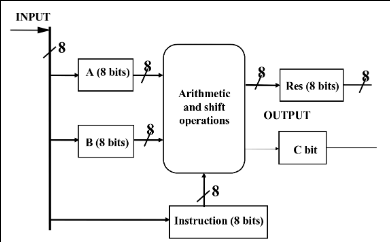
\includegraphics[]{2019-04-08-15-00-51.png}
            PANOPTO 1:21:56
            \medskip

            \begin{figure}[h!]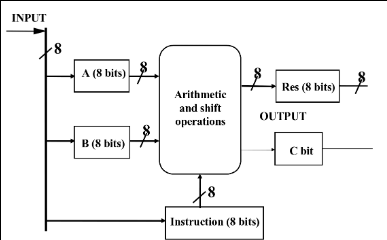
\includegraphics[width=\linewidth]{2019-04-08-20-08-22.png}\end{figure}

            For an $n$-bit ALU, there are $n + 1$ multiplexers, as the last one handles the carry bit. The $C_\text{in}$ bit for the $n^\text{th}$ multiplexer is the $C_\text{out}$ for the $(n - 1)^\text{th}$ multiplexer. The $C_\text{in}$ for the first multiplexer is 0.

\end{document}
